\section{Smooth Structures}
\subsection{Smooth Functions Between Euclidean Spaces}
If $U$ and $V$ are open subsets of $\R^n$ and $\R^m$, a function $F:U \to V$ is called \textbf{smooth} (or $C^\infty$, or infinitely differentiable) if each of its component functions has continuous partial derivatives of all orders. If in addition $F$ is bijective and has a smooth inverse map, it is called a \textbf{diffeomorphism}.
\begin{theorem}[inverse function theorem]
    Suppose $U,V$ are open subsets of $\R^n$, and $F:U \to V$ is a smooth function. If $DF(a)$ is invertible at some point $a \in U$, then there exist connected neighborhoods $U_0 \subset U$ of $a$ and $V_0 \subset V$ of $F(a)$ such that $F|_{U_0}: U_0 \to V_0$ is a diffeomorphism. 
\end{theorem}


\subsection{Smooth Structures on Manifolds}
Let $M$ be a topological $n$-manifold. If $(U, \phe), (V, \psi)$ are two charts such that $U \cap V \neq \varnothing$, the composite map $\psi \circ \phe^{-1}: \phe(U \cap V) \to \psi(U \cap V)$ is called the \textbf{transition map} from $\phe$ to $\psi$. 
Two charts $(U,\phe), (V, \psi)$ are said to be \textbf{smoothly compatible} if either $U \cap V = \varnothing$ or $\psi \circ \phe^{-1}$ is a diffeomorphism. 

Temporarily denote the smooth compatibility of $(U,\phe), (V,\psi)$ by $(U,\phe) \sim (V,\psi)$. Then 
\begin{itemize}
    \item clearly $(U,\phe) \sim (V,\psi)$.  
    \item If $(U,\phe) \sim (V,\psi)$, then $(\psi \circ \phe^{-1})^{-1} = \phe \circ \psi^{-1}$ is still a diffeomorphism, hence $(V, \psi) \sim (U, \phe)$.
    \item Let $(U,\phe) \sim (V,\psi)$ and $(V,\psi) \sim (W,\cta)$, then 
    $\phe \circ \psi^{-1}$ and $\psi \circ \cta^{-1}$ are diffeomorphisms, \\ hence $(\phe \circ \psi^{-1}) \circ (\psi \circ \cta^{-1}) = \phe \circ \cta^{-1}$ is a diffeomorphism, thus $(U,\phe) \sim (W,\cta)$. 
\end{itemize}
We conclude that $\sim$ is an equivalence relation. 
\begin{definition}[atlas]
    We define an \textbf{atlas} for $M$ to be a collection of charts whose domains cover $M$. An atlas $\calA$ is called a \textbf{smooth atlas} if any two charts in $\calA$ are smoothly compatible with each other. 
\end{definition}
\begin{definition}[smooth structure]
    Let $M$ be a topological manifold.
    A smooth atlas $\calA$ on $M$ is \textbf{maximal} if it is not properly contained in any larger smooth atlas. \\
    A \textbf{smooth structure} on $M$ is a maximal smooth atlas. 
\end{definition}

\begin{definition}[smooth manifold]
    A \textbf{smooth manifold} is a pair $(M, \calA)$, where $M$ is a topological manifold and $\calA$ is a smooth structure on $M$. 
\end{definition}

\begin{proposition}[smooth compatibility]
    Let $M$ be a topological manifold.
    \begin{enumerate}
    \item Every smooth atlas $\calA$ for $M$ is contained in a unique maximal smooth atlas, called the \textbf{smooth structure determined by $\calA$}.
    \item Two smooth atlases for $M$ determine the same smooth structure if and only if their union is a smooth atlas. 
    \end{enumerate}
\end{proposition}
\begin{proof}
\begin{enumerate}
    \item Let $\calA$ be a smooth atlas for $M$, and let $\cl{\calA}$ be the set of all charts that are smoothly compatible with every chart in $\calA$. Then clearly $\calA \subset \cl{\calA}$. 
    We need to show that for any $(U,\phe), (V,\psi) \in \cl{\calA}$, the map $\psi \circ \phe^{-1}: \phe(U \cap V) \to \psi(U \cap V)$ is smooth. \\
    Let $x = \phe(p) \in \phe(U \cap V)$ be arbitrary. Since the domains of the charts in $\calA$ cover $M$, there exists a chart $(W, \cta) \in \calA$ such that $p \in W$. Because every chart in $\cl{\calA}$ is smoothly compatible with $(W, \cta)$, the maps $\cta \circ \inv{\phe}$ and $\psi \circ \inv{\cta}$ are smooth. Since $p \in U \cap V \cap W$, it follows that $\psi \circ \inv{\phe} = (\psi \circ \inv{\cta}) \circ (\psi \circ \inv{\cta})$ is smooth on a neighborhood of $x$. Thus $\psi \circ \inv{\phe}$ is smooth in a neighborhood of each point in $\phe(U \cap V)$. Therefore $\cl{\calA}$ is a smooth atlas. If $\cl{\calA}$ is properly contained in a larger smooth atlas $\calE$, then there is a smooth chart $(U, \phe) \in \calE \setminus \cl{\calA}$ which is not compatible with a chart $(V,\psi) \in \calA$. But $\calA \subset \cl{\calA} \subset \calE$ implies $(U, \phe)$ is compatible with $(V,\psi)$, a contradiction. This shows the maximality of $\cl{\calA}$. 
    If $\calB$ is any other maximal smooth atlas containing $\calA$, each of its charts is smoothly compatible with each chart in $\calA$, so $\calB \subset \cl{\calA}$. Since $\calB$ is maximal, $\calB = \cl{\calA}$. 
    \item Let $\calA, \calB$ be smooth atlases for $M$. \\
    ($\Longrightarrow$): Suppose they determine the same smooth structure, then $\calA$ and $\calB$ are contained in a unique maximal smooth atlas $\cl{\calM}$.
    By the construction in (1), every chart in $\cl{\calM}$ is compatible with every chart in $\calA \cup \calB$. 
    
    To show $\calA \cup \calB$ is a smooth atlas, we need to show that for any $(U,\phe), (V,\psi) \in \calA \cup \calB$, the map $\psi \circ \inv{\phe}: \phe(U \cap V) \to \psi(U \cap V)$ is smooth. If $(U,\phe), (V,\psi) \in \calA$ or $(U,\phe), (V,\psi) \in \calB$, then this is the same as part (1). We may assume $(U,\phe) \in \calA$ and $(V,\psi) \in \calB$. 
    If $\calA \cap \calB = \varnothing$, then $U \cap V = \varnothing$, so by definition they are smoothly compatible, implying that $\calA \cup \calB$ is a smooth atlas. Now suppose $\calA \cap \calB \neq \varnothing$ and $U \cap V \neq \varnothing$. Let $x = \phe(p) \in \phe(U \cap V)$ be arbitrary, then there exists a chart $(W,\cta) \in \calA$ with $p \in W$. Because every chart in $\cl{\calM} \supset \calA \cup \calB$ is smoothly compatible with $(W,\cta)$, the maps $\cta \circ \phe^{-1}$ and $\psi \circ \cta^{-1}$ are smooth. The following is the same as part (1). \\
    ($\Longleftrightarrow$): Suppose $\calA$ and $\calB$ determine different smooth structures $\cl{\calA}$ and $\cl{\calB}$, then there is a smooth chart $(U,\phe) \in \cl{\calA}$ such that $(U,\phe) \notin \cl{\calB}$. Then $(U,\phe)$ is smoothly compatible with each $(A,\a) \in \calA$, and there exists $(V,\psi) \in \calB$ with which $(U,\phe)$ is not compatible. 
    Since smooth compatibility is an equivalence relation, $(A,\a)$ is not smoothly compatible with $(V,\psi)$, thus $\calA \cup \calB$ is not a smooth atlas. \qed 
    \end{enumerate}
\end{proof}


\subsection{Local Coordinate Representations}
If $M$ is a smooth manifold, any chart $(U,\phe)$ contained in the given maximal smooth atlas is called a \textbf{smooth chart}, and the coordinate map $\phe$ is called a \textbf{smooth coordinate map}. The domain of a smooth coordinate chart is called a \textbf{smooth coordinate domain} or \textbf{smooth coordinate neighborhood}.

If the image of a smooth coordinate domain under a smooth coordinate map is a ball in Euclidean space, the domain is called a \textbf{smooth coordinate ball}. A \textbf{smooth coordinate cube} is defined similarly. 
\begin{definition}
    We say a set $B \subset M$ is a \textbf{regular coordinate ball} if there is a smooth coordinate ball $B' \supset \cl{B}$ and a smooth coordinate map $\phe:B' \to \R^n$ such that for some positive real numbers $r > r'$:
    $$\phe(B) = B_r(0), \quad \phe(\cl{B}) = \cl{B}_r(0), \quad \phe(B') = B_{r'}(0). $$
\end{definition}
\begin{proposition}
    Every smooth manifold has a countable basis of regular coordinate balls. 
\end{proposition}
\section{Examples of Smooth Manifolds}
\begin{example}
    A topological manifold $M$ of dimension $0$ is just a countable discrete space. 
    For each $p \in M$ the only neighborhood of $p$ that is homeomorphic to an open subset of $\R^0$ is $\{p\}$ itself, and there is exactly one coordinate map $\phe: \{p\} \to \R^0$. 
\end{example}
\begin{example}[~(Euclidean spaces)]
    $\R^n$ is a smooth $n$-manifold with the smooth structure determined by the atlas consisting of the single chart $(\R^n, \id_{\R^n})$. We call this the \textbf{standard smooth structure} on $\R^n$ and the resulting coordinate map \textbf{standard coordinates}. 
\end{example}
\begin{example}[~(another smooth structure on $\R$)]
    Consider the homeomorphism $\psi: \R \to \R$ given by $\psi(x) = x^3$.
    The atlas consisting of the single chart $(\R,\psi)$ defines a smooth structure on $\R$. 
\end{example}
\begin{example}[~(finite-dimensional vector space)]
    Let $V$ be a finite-dimensional real vector space. Any norm on $V$ determines a topology. With this topology, $V$ is a topological $n$-manifold, and has a natural smooth structure defined as follows. Each basis $e_1, \cdots, e_n$ of $V$ defines a basis isomorphism $E: \R^n \to V$ by 
    $$E(x) = \Sum{i=1}{n}x^i e_i. $$
    This map is clearly a homeomorphism, so $(V, E^{-1})$ is a chart. 
    If $\Tilde{e}_1, \cdots, \Tilde{e}_n$ is any other basis and $\Tilde{E}(x) = \Sum{j=1}{n}x^j \Tilde{e}_j$ is the corresponding isomorphism, then there is an invertible matrix $(A_i^j)$ such that $e_i = \Sum{j=1}{n}A_i^j \Tilde{e}_j$ for each $i$. 

    The transition map between the two charts is given by $\Tilde{E}^{-1} \circ E(x) = \Tilde{x}$, where $\Tilde{x} = (\Tilde{x}^1, \cdots, \Tilde{x}^n)$ is determined by
    $$\Sum{j=1}{n}\Tilde{x}^j \Tilde{e}_j = \Sum{i=1}{n}x^i E_i = \Sum{i=1}{n} x^i \Sum{j=1}{n}A_i^j \Tilde{e}_j.$$
    It follows that $\Tilde{x}^j = \Sum{j=1}{n}A_i^j \Tilde{e}_j$, thus $\Tilde{E}^{-1} \circ E$ is an invertible linear map and hence a diffeomorphism, so any two such charts are smoothly compatible. The collection of all such charts thus defines a smooth structure. 
\end{example}

\begin{example}[~(graphs of continuous functions)]
% f:R^2 \to R 最简单的二元函数 参数曲面
    Let $U \subset \R^n$ be an open set, let $f:U \to \R^k$ be a continuous function. The \textbf{graph} of $f$ is the subset of $\R^n \times \R^k$ is defined by 
    $$\Ga(f) = \{(x,y) \in \R^n \times \R^k: y = f(x)\}$$
    with the subspace topology. 
    Let $\pi_1: \R^n \times \R^k \to \R^n$ be the projection onto the first factor, and let $\phe = \pi_1|_{\Ga(f)}$:
    $$\phe(x,y) = x, \quad (x,y) \in \Ga(f). $$
    Then
    \begin{itemize}
        \item $\phe$ is continuous, 
        \item $\phe$ is a homeomorphism since $\phe^{-1}(x) = (x,f(x))$. 
    \end{itemize}
    Thus $\Ga(f)$ is homeomorphic to $\phe(\Ga(f)) = U \subset \R^n$, 
    so $\Ga(f)$ is a topological manifold of dimension $n$. \\
    $(\Ga(f), \phe)$ is a global coordinate chart, called \textbf{graph coordinates}. 

    In summary, the graph of a continuous function is a topological manifold. 
\end{example}
\subsection*{Spheres}
\begin{example}[~(spheres)]
    For each $n \in \N$, the unit $n$-sphere $\S^n$ is Hausdorff and second countable since it is a topological subspace of $\R^{n+1}$. We want to show $\S^n$ is locally Euclidean. For each $i=1, \cdots, n+1$, let
    $$U_i^+ = \{(x_1, \cdots, x_{n+1}) \in \R^{n+1}: x_i > 0 \}, $$
    $$U_i^- = \{(x_1, \cdots, x_{n+1}) \in \R^{n+1}: x_i < 0 \}. $$
    Let $f: \B^n \to \R$ be the continuous function (Notice: $\B^n \subset \R^n$)
    $$f(u) = \sqrt{1-|u|^2}. $$
    The equation of the sphere is given by (temporarily using subscripts) 
    $$x_1^2 + \cdots + x_{n+1}^2=1, $$
    hence 
    $$x_i^2 = 1-x_1^2-\cdots-x_{i-1}^2-x_{i+1}^2-\cdots-x_{n+1}^2, $$
    thus 
    $$x_1^2 + \cdots + x_{i-1}^2 + x_{i+1}^2 + x_{n+1}^2 \leq 1 
    \quad (\text{so that }(x_1, \cdots, x_{i-1}, x_{i+1}, \cdots, x_{n+1}) \in \B^n) $$ 
    and $$x^i = \pm \sqrt{1-x_1^2-\cdots-x_{i-1}^2-x_{i+1}^2-\cdots-x_{n+1}^2} = \pm f((x^1, \cdots, x^{i-1}, x^{i+1}, \dots, x^{n+1})). $$
    Therefore $U_i^+ \cap \S^n$ is the graph of the function\footnote{think $U_i^\pm \cap \S^n$ of north and south hemisphere}
    $$x^i = f(x^1, \cdots, \hat{x^i}, \cdots, x^{n+1}), $$
    where $(x^1, \cdots, \hat{x^i}, \cdots, x^{n+1}):=
    (x^1, \cdots, x^{i-1}, x^{i+1}, \dots, x^{n+1})$. 
    Similarly, $U_i^- \cap \S^n$ is the graph of 
    $$x^i = -f(x^1, \cdots, \hat{x^i}, \cdots, x^{n+1}). $$
    Thus, each $U_i^\pm \cap \S^n$ is locally Euclidean of dimension $n$. The maps $\phe_i^\pm: U_i^\pm \cap \S^n \to \B^n$ given by 
    $$\phe_i^\pm(x^1, \cdots, x^{n+1}) = (x^1, \cdots, \hat{x^i}, \cdots, x^{n+1})$$
    are graph coordinates for $\S^n$. Since each point of $\S^n$ is in the domain of at least one of these $2n+2$ charts, $\S^n$ is a topological $n$-manifold (See Example \ref{1-sphere} for the case $n=1$).
    
\end{example}
\subsection*{Real Projective Spaces}
$\RP^n$ is the quotient space of $\R^{n+1} \setminus \{0\}$ under the equivalence relation
\begin{center}
    $x \sim y$ iff $y=tx$ for some $t \in \R \setminus \{0\}$.
\end{center}
The equivalence class of a point $(a_0, \cdots, a_n) \in \R^{n+1} \setminus \{0\}$ is denoted by $[a_0, \cdots, a_n]$, called the homogeneous coordinates on $\RP^n$. 

%Let $[a_0, \cdots, a_n]$ be the homogeneous coordinates on $\RP^n$. 
In $\R^3$, if $a_0 = 0$, then $[a_0, a_1, a_2]$ is the $x$-axis. In fact, the condition $a_0 \neq 0$ is independent of the choice of a representative for $[a_0, \cdots, a_n]$.

We may define 
$$U_0 = \{[a_0,\cdots,a_n] \in \RP^n : a_0 \neq 0 \}.$$
Similarly, for each $i = 1, \cdots, n$ let 
$$U_i = \{[a_0, \cdots, a_n] \in \RP^n: a_i \neq 0\}. $$
Define 
\begin{align*}
    \phi_0:U_0 &\to \R^n \\
    [a_0, \cdots, a_n] &\mapsto \br{\frac{a_1}{a_0}, \cdots, \frac{a_n}{a_0}}.
\end{align*}
This map has a continuous inverse
$$(b_1, \cdots, b_n) \mapsto [1,b_1, \cdots, b_n]$$
and is therefore a homeomorphism. Similarly, there are homeomorphisms for each $i=1, \cdots, n$:
\begin{align*}
    \phi_0:U_i &\to \R^n \\
    [a_0, \cdots, a_n] &\mapsto \br{\frac{a_1}{a_i}, \cdots, \frac{a_{i-1}}{a_i}, \frac{a_{i+1}}{a_i}, \cdots, \frac{a_n}{a_i}} = \br{\frac{a_1}{a_i}, \hat{\frac{a_i}{a_i}}, \cdots, \frac{a_n}{a_i}}.
\end{align*}
This shows $\RP^n$ is locally Euclidean with the $(U_i,\phi_i)$ as charts. 


\subsection*{Grassman manifolds}
\begin{example}[~(Grassman manifolds)]
    Let $V$ be a real vector space and $\dim V = d < \infty$, the \textbf{Grassmannian} 
    $\Gr_k(V)$ is the set of $k$-dimensional vector subspaces of $V$. 
\end{example}




\subsection*{The Einstein Summation Convention}
We often abbreviate expressions such as $\sum_i x^i e_i$ to $x^i e_i$. This is a rule called the \textbf{Einstein summation convention}. 

\section{Smooth Functions}
\subsection{Smooth Functions on Manifolds}
Suppose $M$ is a smooth $n$-manifold, $k \in \N^+$, $f:M \to \R^k$ is any function. \begin{definition}[smooth function]
    We say that $f$ is a \textbf{smooth function} if for every $p \in M$ there exists a smooth chart $(U, \phe)$ for $M$ whose domain contains $p$ and such that 
    \begin{center}
        $f \circ \phe^{-1}$ is smooth on $\phe(U) \subset \R^n$. 
    \end{center}
\end{definition}
\begin{exercise}
    Let $M$ be a smooth manifold with or without boundary. Show that pointwise multiplication turns $C^{\infty}(M)$ into a commutative ring and a commutative and associative algebra over $\mathbb{R}$. (See Appendix B, p. 624, for the definition of an algebra.)
\end{exercise}
\begin{proof}
    Let $f,g \in C^\infty(M)$, then clearly $(C^\infty(M), +)$ is an abelian group. Multiplicative associativity is obvious, so it remains to show $fg \in C^\infty(M)$. By definition, there are smooth charts near a point $(U, \phe), (V, \psi)$ near a point $p \in M$ such that 
    $f \circ \phe^{-1}$ is smooth on $\phe(U)$ and $g \circ \psi^{-1}$ is smooth on $\psi(V)$. 
\end{proof}
%\begin{exercise}
    %Let $U$ be an open submanifold of $\mathbb{R}^n$ with its standard smooth manifold structure. Show that a function $f: U \rightarrow \mathbb{R}^k$ is smooth in the sense just defined if and only if it is smooth in the sense of ordinary calculus. Do the same for an open submanifold with boundary in $\mathbb{H}^n$ (see Exercise 1.44).
%\end{exercise}
\begin{exercise}
    Let $M$ be a smooth manifold with or without boundary, and suppose $f: M \rightarrow \mathbb{R}^k$ is a smooth function. Show that $f \circ \varphi^{-1}: \varphi(U) \rightarrow \mathbb{R}^k$ is smooth for every smooth chart $(U, \varphi)$ for $M$.
\end{exercise}
\begin{proof}
    Recall that any two smooth charts are smoothly compatible. 
    Let $(U,\phe)$ be an arbitrary smooth chart and let $p \in U$. Then for this $p$ there exists a smooth chart $(V,\psi)$ such that $V \ni p$ and $f \circ \psi^{-1}$ is smooth on $\psi(U)$. Since $(U,\phe)$ is smoothly compatible with $(V,\psi)$, 
    $\psi \circ \phe^{-1}$ is a diffeomorphism. Now
    $$f \circ \phe^{-1} = (f \circ \psi^{-1}) \circ (\psi \circ \phe^{-1}) $$
    is smooth on $\phe(U)$, so $f$ is a smooth function. \qed 
\end{proof}

\begin{definition}[coordinate representation]
    Given a function $f:M \to \R^k$ and a chart $(U, \phe)$ for $M$, the function $\hat{f}: \phe(U) \to \R^k$ defined by $\hat{f}(x) = f \circ \phe^{-1}(x)$ is called the \textbf{coordinate representation} of $f$. 
\end{definition}
\begin{example}
    Consider $f(x,y)=x^2+y^2$ defined on $\R^2$. In polar coordinates on the set $U=\{(x,y):x>0\}$, it has the coordinate representation $\hat{f}(r,\cta) = r^2$.
\end{example}
\subsection{Smooth Maps Between Manifolds}
\begin{definition}[smooth map]
    Let $M,N$ be smooth manifolds, $F:M \to N$ be any map. 
    We say that $F$ is a \textbf{smooth map} if for every $p \in M$, there exists smooth charts $(U, \phe)$ containing $p$ and $(V, \psi)$ containing $F(p)$ such that 
    \begin{itemize}
        \item $F(U) \subset V$, and 
        \item $\psi \circ F \circ \phe^{-1}$ is smooth from $\phe(U)$ to $\psi(V)$. 
    \end{itemize}
\end{definition}
\begin{proposition}
    Every smooth map is continuous. 
\end{proposition}
\begin{proof}
    Let $M,N$ be smooth  manifolds and $F:M \to N$ be smooth. Let $p \in M$, then there are smooth charts $(U,\phe)$ containing $p$ and $(V,\psi)$ containing $F(p)$ such that $F(U) \subset V$ and 
    $\psi \circ F \circ \phe^{-1}: \phe(U) \to \psi(V)$ 
    is a smooth function, hence is continuous. Then 
    $$F|_U = \psi^{-1} \circ (\psi \circ F \circ \phe^{-1}) \circ \phe: U \to V$$
    is continuous in a neighborhood of $p$. Since $p$ is arbitrary, $F$ is continuous on $M$. \qed 
\end{proof}


\begin{proposition}
    Let $M$ and $N$ be smooth manifolds and let $F:M \to N$ be a map. 
    \begin{enumerate}
    \item If every $p \in M$ has a neighborhood $U$ such that $F|_U$ is smooth, then $F$ is smooth. 
    \item If $F$ is smooth, then its restriction to every open subset is smooth. 
    \end{enumerate}
\end{proposition}
\begin{proof}
    \begin{enumerate}
    \item Let $p \in M$, then there are smooth charts $(U,\phe)$ containing $p$ and $(V,\psi)$ containing $F|_U(p)$ such that $F|_U(U) \subset V$ and 
    $\psi \circ F|_U \circ \phe^{-1}: \phe(U) \to \psi(V)$ 
    is a smooth function. It is obvious that $F|_U(U) = F(U)$, so all $F|_U$'s appeared in the above expressions can be substituted by $F$, thus $F$ is smooth. 
    \item Let $W$ be an open set in $M$. 
    %Then it suffices to show that for every $p \in W$ there exists smooth charts $(U_p, \phe_p)$ and $(V_p, \psi_p)$ such that $F|_U(U_p) \subset V_p$ and $\psi_p \circ F|_U \circ \phe^{-1}$ is smooth from $\phe(U)$ to $\psi(V)$. 
    By the smoothness of $F$, for every $p \in W$ there exists smooth charts $(U_p, \phe_p)$ and $(V_p, \psi_p)$ such that $F(U_p) \subset V_p$ and $\psi_p \circ F \circ \phe^{-1}$ is smooth from $\phe(U)$ to $\psi(V)$.
    By considering the set $W \cap U_p$ it is easy to see that $F|_W$ is smooth. 
    % 如何从任意跨到存
    \end{enumerate} \qed 
\end{proof}
\begin{theorem}[gluing lemma]
    Let $M,N$ be smooth manifolds and $\{U_\a\}_{\a \in A}$ be an open cover of $M$. Suppose for each $\a$ we are given a smooth map $F_\a:U_\a \to N$ such that 
    $$F_\a|_{U_\a \cap U_\b} = F_\b|_{U_\a \cap U_\b}~\forall \a, \b.$$
    Then there exists a unique smooth map $F:M \to N$ such that 
    $$F|_{U_\a} = F_\a~\forall \a \in A. $$
\end{theorem}

A smooth map $F:M \to N$ induces a smooth structure on $N$.
\begin{theorem}
    Let $\{(U, \phe)\}$ be a smooth structure on $M$, then 
    $\{(F(U), \}$ is a smooth structure on $N$. 
\end{theorem}


\subsection{Diffeomorphisms}
\begin{definition}
    If $M,N$ are smooth manifolds, a \textbf{diffeomorphism} from $M$ to $N$ is a smooth bijective map $F:M \to N$ that has a smooth inverse. We say that $M$ and $N$ are \textbf{diffeomorphic} if there exists a diffeomorphism between them. 
\end{definition}
\begin{example}
    Let $F: \B^n \to \R^n$ and $G: \R^n \to \B^n$ be
    $$F(x) = \frac{x}{\sqrt{1-|x|^2}}, \quad G(y) = \frac{y}{\sqrt{1+|y|^2}}. $$
    Then $F,G$ are diffeomorphisms. 
\end{example}
\begin{proof}
    First we compute $F \circ G$ and $G \circ F$. 
    $$(F \circ G)(y) = F(G(y)) = \frac{G(y)}{\sqrt{1-|G(y)|^2}}, $$
    where $$1-|G(y)|^2 = 1-\frac{|y|^2}{1+|y|^2} = \frac{1}{1+|y|^2},$$
    hence $$(F \circ G)(y) = \frac{y}{\sqrt{1+|y|^2}} / \frac{1}{\sqrt{1+|y|^2}} = y. $$ Similarly, $$(G \circ F) (x) = x. $$
    Now consider each component $F_i(x) = \frac{x_i}{\sqrt{1-|x|^2}}$, then $F_i$ is smooth by elementary calculus. Hence $\B^n$ is diffeomorphic to $\R^n$. \qed 
\end{proof}
\begin{example}
    If $M$ is a smooth manifold and $(U,\phe)$ is a smooth coordinate chart on $M$, then $\phe:U \to \phe(U) \subset \R^n$ is a diffeomorphism.   
\end{example}
\begin{proof}
    Since $\phe \circ \phe^{-1} = \id$ is clearly smooth, $\phe$ is a smooth map. To see $\phe^{-1}$ is smooth, we view $\phe^{-1}$ as a map between manifolds $\R^n$ and $M$. Choose a smooth chart $(\phe(U), \phe^{-1})$ on $\R$, then $\phe^{-1} \circ (\phe^{-1})^{-1} = \id$ is clearly smooth, completing the proof.   
\end{proof}

\begin{proposition}[properties of diffeomorphisms]
Let $M,N,P$ be manifolds. 
    \begin{enumerate}
        \item If $F: M \to N, G: N \to P$ are diffeomorphisms, then $G \circ F:M \to P$ is a diffeomorphism. 
        \item If $F, G$ are diffeomorphisms from $M$ to $N$, 
        then the Cartesian product $F \times G$ is a diffeomorphism. 
        \item ``Diffeomorphic" is an equivalence relation on the class of all smooth manifolds. 
    \end{enumerate}
\end{proposition}
\begin{proof}
    \begin{enumerate}
    \item Let $p \in M$. Since $F$ is smooth, there are smooth charts $(U, \phe)$ on $M$ and $(V_F, \psi)$ on $N$ such that $p \in U, F(U) \subset V_F$ and $\psi \circ F \circ \phe^{-1}:\phe(U) \to \psi(V_F)$ is a smooth function. 
    Since $G$ is smooth, $G|_{F(U)}$ is smooth, so there are smooth charts $(F(U), \psi)$ on $N$ and $(W, \xi)$ on $P$ such that 
    \begin{itemize}
        \item $F(p) \in F(U), (G \circ F) (p) \in G(F(U)) \subset W$, 
        \item $\xi \circ G \circ \psi^{-1}$ is a smooth function. 
    \end{itemize}
    Then 
    $$\xi \circ G \circ \psi^{-1} \circ \psi \circ F \circ \phe^{-1} 
      = \xi \circ (G \circ F) \circ \phe^{-1} : \phe(U) \to \xi(W) $$
    is a smooth function, hence $G \circ F$ is a diffeomorphism. 
    \begin{figure}[h]
        \centering
        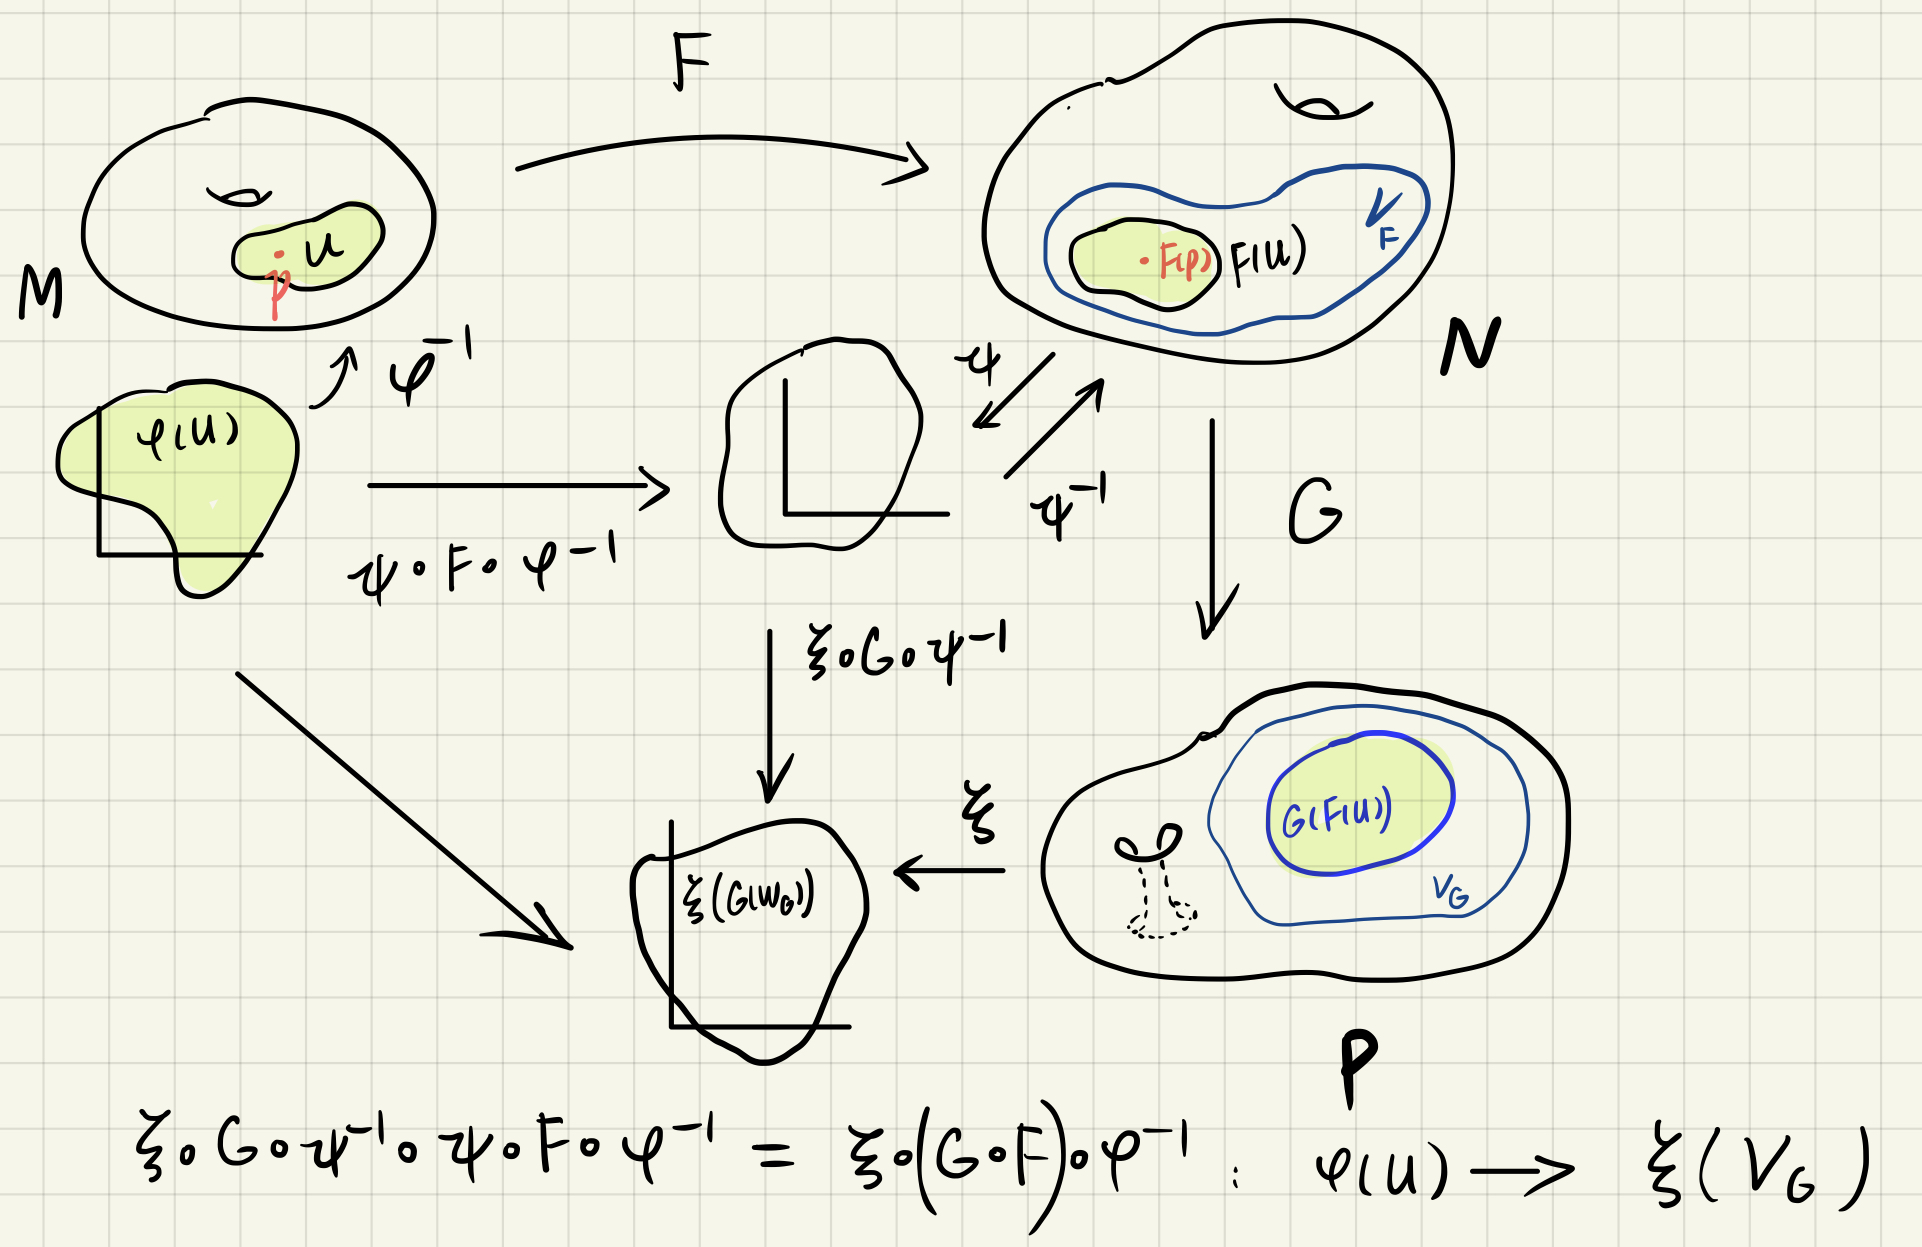
\includegraphics[scale=0.2]{figure/Lee2.15.jpeg}
    \end{figure}
    
    \item Let $p \in M$, then there are smooth charts $(U_F, \phe_F), (U_G, \phe_G)$ and $(V_F, \psi_F), (V_G, \psi_G)$ such that 
    \begin{itemize}
        \item $p \in U_f, p \in U_G$ and $F(p) \in V_F, G(p) \in V_G$,
        \item $\psi_F \circ F \circ \phe_F^{-1}$ and $\psi_G \circ G \circ \phe_G^{-1}$ are smooth functions. 
    \end{itemize}
    % 什么是product of diffeomorphisms???
    \item Let $M, N, P$ be smooth manifolds. 
    \begin{itemize}
        \item $M$ is clearly diffeomorphic with $M$ via the identity map. 
        \item If $F:M \to N$ is a diffeomorphism, so is $F^{-1}: N \to M$. 
        \item Suppose $M \simeq N$ and $N \simeq P$. Since composition of diffeomorphisms is a diffeomorphism, $M \simeq P$.
    \end{itemize}
    \end{enumerate} \qed 
\end{proof}

\section{Partitions of Unity}
\begin{lemma}
    The function $f:\R \to \R$ given by 
    $$f(t) = \begin{cases}
    e^{-1/t}, &t > 0, \\
    0,        &t \leq 0, \end{cases}$$
    is smooth. 
\end{lemma}
\begin{proof}
    This is a calculus exercise. \qed 
\end{proof}
\begin{lemma}
    For any $0 < r_1 < r_2$ there is a smooth functions $h: \R^n \to \R$, where 
    \begin{enumerate}
    \item $H = 1$ on $\cl{B_{r_1}(0)}$;
    \item $0<H<1$ on $B_{r_2}(0) \setminus \cl{B_{r_1}(0)}$;
    \item $H = 0$ on $\R^n \setminus B_{r_2}(0)$.
    \end{enumerate}
    Using the notation in Urysohn's lemma, we can write 
    $$\cl{B_{r_1}(0)} \prec h \prec B_{r_2}(0). $$
\end{lemma}
\begin{proof}
    Let  $$f(t) = \begin{cases}
    e^{-1/t}, &t > 0, \\
    0,        &t \leq 0, \end{cases}$$
    and define 
    $$ H(x) = \frac{f(r_2 - |x|)}{f(r_2 - |x|) + f(|x| - r_1)}. $$
    Then
    \begin{enumerate}
    \item If $x \in \cl{B_{r_1}(0)}$, then $0 \leq |x| \leq r_1 < r_2$, so
    $f(|x|-r_1) = 0$, hence $H(x) = f(r_2-|x|) / f(r_2-|x|) = 1$.
    \item Let $x \in B_{r_2}(0) \setminus \cl{B_{r_1}(0)}$, then $r_1 < |x| < r_2$, so $f(r_2 - |x|) > 0$ and $f(|x|-r_1) > 0$, hence $0 < H(x) < 1$.
    \item If $x \in \R^n \setminus B_{r_2}(0)$, then $|x| \geq r_2$, so $f(r_2 - |x|) = 0$.
    \end{enumerate}
    Therefore $H$ is as desired. \qed 
\end{proof}

\begin{definition}
    Let $M$ be a topological space, $\calX=(X_\a)_{\a \in A}$ be an open cover of $M$. A \textbf{partition of unity} subordinate to $\calX$ is a family $\{\psi_\a\}_{\a \in A}$ of continuous functions $\psi_\a:M \to \R$ with the following properties:
    \begin{enumerate}
    \item $0 \leq \psi_\a(x) \leq 1 ~\forall \a \in A$ and $\forall x \in M$.
    \item $\supp (\psi_\a) \subset X_\a$ for each $\a \in A$. 
    \item $\{\supp (\psi_\a)\}_{\a \in A}$ is locally finite.
    \item $\sum_{\a \in A} \psi_\a(x) = 1$ for all $x \in M$. 
    \end{enumerate}
    If $M$ is a smooth manifold and each $\psi_\a$ is smooth, then $\{\psi_\a\}_{\a \in A}$ is called a smooth partition of unity. 
\end{definition}

\begin{theorem}\label{Lee2.23}
    Suppose $M$ is a smooth manifold and $\calX = (X_\a)_{\a \in A}$ is an open cover of $M$. Then there exists a smooth partition of unity subordinate to $\calX$. 
\end{theorem}

If $M$ is a topological space, $A \subset M$ is a closed set, $U \supset A$ is open, a continuous function $\psi:M \to \R$ is called a \textbf{bump function} for $A$ supported in $U$ if $\psi = 1$ on $A$, $\supp \psi \subset U$, and $0 \leq \psi \leq 1$. Analysts use the notation $A \prec f \prec U$ to describe the above properties. 
\begin{proposition}\label{Lee2.25}
    Let $M$ be a smooth manifold. For any closed $A \subset M$ and any open $U \supset A$, there exists a smooth bump function for $A$ supported in $U$. 
\end{proposition}
\begin{proof}
    Let $U_0 = U$ and $U_1 = M \setminus A$, and let $\{\psi_0, \psi_1\}$ be a smooth partition of unity subordinate to the open cover $\{U_0, U_1\}$. Since $\psi_0 = 0$ on $A$, it follows that $\psi_0 = \sum_i \psi_i = 1$ there, the function $\psi_0$ has the desired properties. \qed 
\end{proof}
\begin{lemma}[extension lemma]
    Suppose $M$ is a smooth manifold, $A \subset M$ is closed, $f:A \to \R^k$ is a smooth function. Then for any open $U \supset A$, there is a smooth function $\Tilde{f}:M \to \R^k$ such that $\Tilde{f}|_A = f$ and $\supp \Tilde{f} \subset U$. 
\end{lemma}

% input in smoothness.tex

\section{Manifolds with Boundary}
We define the \textbf{closed $n$-dimensional upper half-space} $\H^n = \{(x^1, \cdots, x^n) \in \R^n: x^n \geq 0\}$. When $n>0$, the interior and boundary of $\H^n$ are given by 
\begin{align*}
    \Int \H^n &= \{(x^1, \cdots, x^n) \in \R^n: x^n > 0\},       \\
    \partial \H^n &= \{(x^1, \cdots, x^n) \in \R^n: x^n = 0\}.
\end{align*}
In the $n=0$ case, $\H^0 = \R^0 = \{0\}$, so $\Int H^0 = \R^0$ and $\partial \H^0 = \varnothing$. 